\subsection{Topologia del Sistema}

La topologia del sistema è rappresentata nel seguente schema:

\begin{figure}[h]
\centering
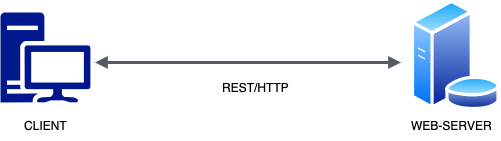
\includegraphics[scale=0.75]{images/topologia.png}
\caption{Diagramma dell’architettura della webapp Spendly}
\end{figure}


Il sistema è basato su un’architettura \textbf{Client-Server}, in cui i client interagiscono con un \textbf{web server} sviluppato utilizzando il framework \textbf{Spring Boot}. I client possono essere:

\begin{itemize}
\item \textbf{Applicazione Web}: gli utenti accedono a Spendly tramite un browser, comunicando con il server attraverso \textbf{API REST/HTTP}.
\item \textbf{Applicazione Mobile}: gli utenti interagiscono con il sistema tramite un’app mobile che utilizza \textbf{REST/HTTP} per le richieste e \textbf{SMTP} per le notifiche via email.
\end{itemize}


Il \textbf{web server}, sviluppato con \textbf{Spring Boot}, gestisce le richieste dei client e include al suo interno il database \textbf{PostgreSQL}, che garantisce la persistenza e la gestione efficiente dei dati. Questa integrazione semplifica la gestione delle risorse e riduce la latenza nelle operazioni di lettura e scrittura.

\subsubsection{Gestione delle comunicazioni}
Il sistema utilizza il protocollo \textbf{REST/HTTP} per lo scambio di dati in formato \textbf{JSON}, assicurando l’interoperabilità tra diverse piattaforme. Per l’invio delle notifiche agli utenti, viene impiegato il protocollo \textbf{SMTP}.

\subsubsection{Caratteristiche dell’architettura}

\begin{itemize}
\item \textbf{Scalabilità}: possibilità di scalare l’intero sistema o le singole funzionalità in base alle necessità.
\item \textbf{Modularità}: sviluppo e manutenzione semplificati grazie all’organizzazione delle funzionalità in moduli indipendenti.
\item \textbf{Affidabilità}: eventuali malfunzionamenti in una funzionalità non compromettono l’intero sistema.
\item \textbf{Manutenibilità}: possibilità di aggiornare o sostituire singoli moduli senza interrompere l’operatività complessiva.
\end{itemize}